\section{Abuse Cases}
\label{sec:abuse_cases}

Bei der Lösung handelt es sich um ein verteiltes System, das über unsichere Netze kommuniziert. Daraus ergeben sich Angriffspunkte, auf die bei der Umsetzung besonders geachtet werden muss.

\begin{figure}
  \centering
    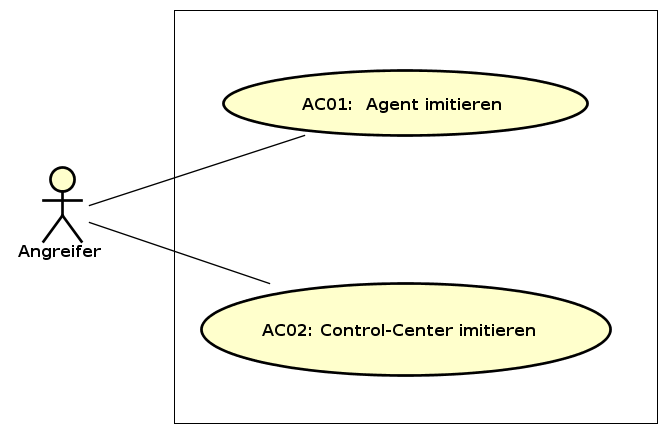
\includegraphics[width=0.6\textwidth]{files/AbuseCases_small}
  \caption{Übersicht der Abuse Cases}
  \label{fig:abusecases}
\end{figure}

\subsection*{AC01: Agent imitieren}
\label{auc:01}

    Szenario: Ein Angreifer gibt sich als Agent aus und meldet sich beim \gls{controlcenter} an. Damit ist es dem Angreifer möglich, verfälschte Daten an das System zu schicken und dem Systemadministrator gezielt falsche Informationen zu vermitteln. Im schlimmsten Fall trifft der Systemadministrator falsche Entscheidungen.

\subsection*{AC02: Control-Center imitieren}
\label{auc:02}

Szenario: Ein Angreifer gibt sich als falsches \gls{controlcenter} aus und meldet sich beim Agent. Der Angreifer kann Aufträge für Software-Updates erteilen und so direkt auf das System Einfluss nehmen.